\section{Threshold of Growth for 2-Connected Components}\label{sec:growth-components}
In this section we prove that for sparse hypergraphs, all 2-connected components have constant size.
\component*

In order to prove the lemma, we formalize the notion of growing a subhypergraph.

\paragraph{Possible 2-neighbors of a sub-hypergraph and Definition of $\grow$.}
In Section~\ref{sec:const-size}, we discussed that the size of 2-connected components can be bounded by examining how 2-connected sub-hypergraphs can grow. Specifically, we will look at a sub-hypergraph $H\subset \rhG$ and the possible ways for $H$ to have a 2-neighbor. 
% \red{check all uses}
% \gb{What's happening here?}



Suppose $\shG$ is a sub-hypergraph of $\rhG$ and $\cli(\proj(\shG))$ is 2-connected. 
Let $N(\shG)$ 
% $N(\shG)\defeq \nei{\chG d}(\cli(\proj(\shG)))$ 
be the set of all possible 2-neighbors of $\cli(\proj(\shG))$. If $\cli(\proj(\shG))$ is a proper subset of a larger 2-connected hypergraph $\cli(\proj(\shG'))$ for some $\shG'\subset \rhG$, then there must exist $\he \in N(\shG)$ that is in $\cli(\proj(\shG'))$. An example is drawn in Figure~\ref{fig:possible-neighbors}, where $\shG$ only contains one hyperedge $\{1,2,3\}$, and all 3 possible 2-neighbors of $\{1,2,3\}$ forms $N(\shG)$.
% \begin{figure}
% \centering
% \begin{tikzpicture}
%     \coordinate (1) at (0,0);
%     \coordinate (2) at (4,0);
%     \coordinate (3) at (2,3.46);
%     \coordinate (4) at (2,-3.46);
%     \coordinate (5) at (-2,3.46);
%     \coordinate (6) at (6,3.46);
%     % Main triangle 123 in the middle

%     % Fill triangle 123 with green
%     \fill[green!30] (1.center) -- (2.center) -- (3.center) -- cycle;
%     \fill[cyan!30] (1.center) -- (2.center) -- (4.center) -- cycle;
%     \fill[cyan!30] (1.center) -- (3.center) -- (5.center) -- cycle;
%     \fill[cyan!30] (3.center) -- (2.center) -- (6.center) -- cycle;
%     \node[draw, circle, fill=black, label=left:1] (1) at (0,0) {};
%     \node[draw, circle, fill=black, label=right:2] (2) at (4,0) {};
%     \node[draw, circle, fill=black, label=above:3] (3) at (2,3.46) {}; % 3.46 approximates sqrt(12) to form an equilateral triangle
    
%     % Additional nodes 4, 5, 6
%     \node[draw, circle, fill=black, label=below:4] (4) at (2,-3.46) {}; % Placed symmetrically below 1
%     \node[draw, circle, fill=black, label=left:5] (5) at (-2,3.46) {}; % Placed symmetrically left of 2
%     \node[draw, circle, fill=black, label=right:6] (6) at (6,3.46) {}; % Placed symmetrically right of 3
    
%     % Dotted line triangles 124, 235, and 136
%     % \draw[dotted] (1) -- (2) -- (4) -- (1);
%     % \draw[dotted] (2) -- (3) -- (6) -- (2);
%     % \draw[dotted] (1) -- (3) -- (5) -- (1);
% \end{tikzpicture}
% \caption{An illustration of $N(\hE)$. Here $\hE$ only has one hyperedge $\{1,2,3\}$, colored in green. $N(\hE)$ contains three possible 2-neighbors of $\cli(\proj(\hE))=\hE$, colored in blue.}
% \label{fig:possible-neighbors}
% \end{figure}

\begin{figure}
\centering
\begin{minipage}{.45\textwidth}

\centering
   % \resizebox{0.7\textwidth}{!}{
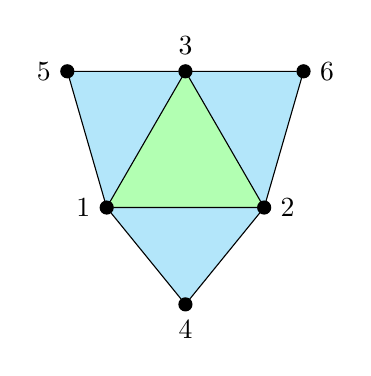
\begin{tikzpicture}[scale=0.50]
    \coordinate (1) at (0,0);
    \coordinate (2) at (4,0);
    \coordinate (3) at (2,3.46);
    \coordinate (4) at (2,-2.46);
    \coordinate (5) at (-1,3.46);
    \coordinate (6) at (5,3.46);
    % Main triangle 123 in the middle

    % Fill triangle 123 with green
    \fill[green!30] (1.center) -- (2.center) -- (3.center) -- cycle;
    \fill[cyan!30] (1.center) -- (2.center) -- (4.center) -- cycle;
    \fill[cyan!30] (1.center) -- (3.center) -- (5.center) -- cycle;
    \fill[cyan!30] (3.center) -- (2.center) -- (6.center) -- cycle;
    \node[draw, circle, fill=black, scale=0.5,label=left:1] (1) at (0,0) {};
    \node[draw, circle, fill=black, scale=0.5,label=right:2] (2) at (4,0) {};
    \node[draw, circle, fill=black, scale=0.5,label=above:3] (3) at (2,3.46) {}; % 3.46 approximates sqrt(12) to form an equilateral triangle
    
    % Additional nodes 4, 5, 6
    \node[draw, circle, fill=black, scale=0.5,label=below:4] (4) at (4) {}; % Placed symmetrically below 1
    \node[draw, circle, fill=black, scale=0.5,label=left:5] (5) at (5) {}; % Placed symmetrically left of 2
    \node[draw, circle, fill=black, scale=0.5,label=right:6] (6) at (6) {}; % Placed symmetrically right of 3
    
    \node at (barycentric cs:1=1,2=1,3=1) {$\shG$};
    
    % Dotted line triangles 124, 235, and 136
    \draw (1) -- (2) -- (4) -- (1);
    \draw (2) -- (3) -- (6) -- (2);
    \draw (1) -- (3) -- (5) -- (1);
\end{tikzpicture}
\caption{An illustration of $N(\shG)$ when $d=3$. Here $\shG$ only has one hyperedge $\{1,2,3\}$, colored in green. $N(\shG)$ contains three possible 2-neighbors of $\cli(\proj(\shG))=\shG$, colored in blue.}
\label{fig:possible-neighbors}
\vspace{12mm}
\end{minipage}%
\hfill
\begin{minipage}{.45\textwidth}
\centering
   % \resizebox{0.7\textwidth}{!}{
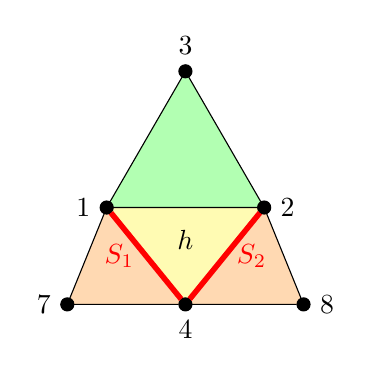
\begin{tikzpicture}[scale=0.50]
    % Define coordinates
    \coordinate (1) at (0,0);
    \coordinate (2) at (4,0);
    \coordinate (3) at (2,3.46);
    \coordinate (4) at (2,-2.46);
    % \coordinate (5) at (-2,3.46);
    % \coordinate (6) at (6,3.46);
    \coordinate (7) at (-1,-2.46); % Additional point to the left
    \coordinate (8) at (5,-2.46); % Additional point to the right
    
    % Fill triangles with respective colors
    \fill[green!30] (1.center) -- (2.center) -- (3.center) -- cycle;
    \fill[yellow!30] (1.center) -- (2.center) -- (4.center) -- cycle; % Refill with yellow
    % \fill[cyan!30] (1.center) -- (3.center) -- (5.center) -- cycle;
    % \fill[cyan!30] (3.center) -- (2.center) -- (6.center) -- cycle;
    \fill[orange!30] (1.center) -- (4.center) -- (7.center) -- cycle; % New triangle 147
    \fill[orange!30] (2.center) -- (4.center) -- (8.center) -- cycle; % New triangle 248
    
    % Draw nodes
    \node[draw, circle, fill=black,scale=0.5, label=left:1] (1) at (1) {};
    \node[draw, circle, fill=black, scale=0.5,label=right:2] (2) at (2) {};
    \node[draw, circle, fill=black, scale=0.5,label=above:3] (3) at (3) {};
    \node[draw, circle, fill=black, scale=0.5,label=below:4] (4) at (4) {};
    % \node[draw, circle, fill=black, label=left:5] (5) at (5) {};
    % \node[draw, circle, fill=black, label=right:6] (6) at (6) {};
    \node[draw, circle, fill=black,scale=0.5, label=left:7] (7) at (7) {};
    \node[draw, circle, fill=black, scale=0.5, label=right:8] (8) at (8) {};
    
    % Dotted line triangles
    \draw (1) -- (2) -- (4) -- (1);
    % \draw (2) -- (3) -- (6) -- (2);
    % \draw (1) -- (3) -- (5) -- (1);
    \draw (1) -- (4) -- (7) -- (1); % Dotted lines for new triangle 147
    \draw (2) -- (4) -- (8) -- (2); % Dotted lines for new triangle 248
    
    % Place "h" in the middle of triangle 124
    \node at (barycentric cs:1=1,2=1,4=1) {$h$};
    \node at (barycentric cs:1=1,2=1,3=1) {$\shG$};
    
    % Color intervals 14 and 24 and add labels
    \draw[line width=2pt, red] (1) -- node[left] {$S_1$} (4);
    \draw[line width=2pt, red] (2) -- node[right] {$S_2$} (4);
    
    % Draw edges for clarity (optional)
    \draw (1) -- (2);
    \draw (1) -- (3);
    \draw (2) -- (3);
\end{tikzpicture}
\caption{An example of an element in $\grow(\shG,\he)$, consists of 3 hyperedges, $\{1,2,3\},\{1,4,7\}\text{ and }\{2,4,8\}$. Here $\shG$ contains one hyperedge $\{1,2,3\}$. $\he=\{1,2,4\}$. For $\he$ to be included in the 2-connected component, one way is to include $S_1^{\shG,\he} = \{1,4\}$ and $S_2^{\shG,\he} = \{2,4\}$ respectively in two hyperedges. }
\label{fig:example-grow}
\end{minipage}
\end{figure}

For $\he\in N(\shG)$ to appear in the 2-connected hypergraph $\cli(\proj(\shG'))$, every edge in $\proj(\he)\backslash \proj(\shG)$ should be covered in at least one hyperedge in $\shG'$.
Now let us examine the possible ways for this to happen.  
Let $\cS^{\shG,\he} \defeq \{S_1^{\shG,\he}, S_2^{\shG,\he}, \cdots, S_m^{\shG,\he}\}$ be the collection of subsets of $\he$ such that $\proj(S_i)\not\subseteq \proj(\shG)$ and $\proj(S_i)\ne \emptyset$. Let $m$ be the number of such subsets, and note that $m\le 2^d$. 
If a hyperedge covers an edge in $\proj(\he)\backslash \proj(\shG)$, it must intersect with $h$ at one of the sets in $\cS^{\shG,\he}$. For any $\he\in N(\shG)$, we define
% \gbdone{change $K$ to $S$ and then can use $K$ later for sub-hypergraph}
\[
    \grow(\shG, \he) \defeq \{\shG\cup(\cup_{i\in I}\{\he_i\}): I\subseteq [m], \he_i\cap \he = S_i^{\shG,\he} , \proj(\cup_{i\in I}S_i^{\shG,\he}) = \proj(h)\backslash \proj(\shG)\}\,,
\]
and
\[
\grow(\shG) \defeq  \bigcup_{\he\in N(\shG)}\grow(\shG)\,.
\]
An example of an element in $ \grow(\shG, \he)$ is shown in Figure~\ref{fig:example-grow}.
% \begin{figure}
% \centering
% \begin{tikzpicture}
%     % Define coordinates
%     \coordinate (1) at (0,0);
%     \coordinate (2) at (4,0);
%     \coordinate (3) at (2,3.46);
%     \coordinate (4) at (2,-3.46);
%     \coordinate (5) at (-2,3.46);
%     \coordinate (6) at (6,3.46);
%     \coordinate (7) at (-3,-3.46); % Additional point to the left
%     \coordinate (8) at (7,-3.46); % Additional point to the right
    
%     % Fill triangles with respective colors
%     \fill[green!30] (1.center) -- (2.center) -- (3.center) -- cycle;
%     \fill[yellow!30] (1.center) -- (2.center) -- (4.center) -- cycle; % Refill with yellow
%     % \fill[cyan!30] (1.center) -- (3.center) -- (5.center) -- cycle;
%     % \fill[cyan!30] (3.center) -- (2.center) -- (6.center) -- cycle;
%     \fill[orange!30] (1.center) -- (4.center) -- (7.center) -- cycle; % New triangle 147
%     \fill[orange!30] (2.center) -- (4.center) -- (8.center) -- cycle; % New triangle 248
    
%     % Draw nodes
%     \node[draw, circle, fill=black, label=left:1] (1) at (1) {};
%     \node[draw, circle, fill=black, label=right:2] (2) at (2) {};
%     \node[draw, circle, fill=black, label=above:3] (3) at (3) {};
%     \node[draw, circle, fill=black, label=below:4] (4) at (4) {};
%     % \node[draw, circle, fill=black, label=left:5] (5) at (5) {};
%     % \node[draw, circle, fill=black, label=right:6] (6) at (6) {};
%     \node[draw, circle, fill=black, label=left:7] (7) at (7) {};
%     \node[draw, circle, fill=black, label=right:8] (8) at (8) {};
    
%     % Dotted line triangles
%     \draw[dotted] (1) -- (2) -- (4) -- (1);
%     % \draw[dotted] (2) -- (3) -- (6) -- (2);
%     % \draw[dotted] (1) -- (3) -- (5) -- (1);
%     \draw[dotted] (1) -- (4) -- (7) -- (1); % Dotted lines for new triangle 147
%     \draw[dotted] (2) -- (4) -- (8) -- (2); % Dotted lines for new triangle 248
    
%     % Place "h" in the middle of triangle 124
%     \node at (barycentric cs:1=1,2=1,4=1) {$h$};
    
%     % Color intervals 14 and 24 and add labels
%     \draw[line width=2pt, red] (1) -- node[left] {$S_1$} (4);
%     \draw[line width=2pt, red] (2) -- node[right] {$S_2$} (4);
    
%     % Draw edges for clarity (optional)
%     \draw (1) -- (2);
%     \draw (1) -- (3);
%     \draw (2) -- (3);
% \end{tikzpicture}
% \caption{An example of an element in $\grow(\hE,\he)$, consists of 3 hyperedges, $\{1,2,3\},\{1,4,7\},\{2,4,8\}$. Here $\hE$ contains one hyperedge $\{1,2,3\}$. $\he=\{1,2,4\}$. For $\he$ to be included in the 2-connected component, one way is to include $S_1^{\shG,\he} = \{1,4\}$ and $S_2^{\shG,\he} = \{2,4\}$ respectively in two hyperedges. }
% \label{fig:example-grow}
% \end{figure}

% Let $\hE_i^\he$ be the set of such hyperedges.
% \[
% \hE_i^\he\defeq \B\{\he'\in \binom{[n]}{d}: \he'\cap \he = S_i^{\shG,\he}\B\}\,
% \]
% \cg{cg: This paragraph is probably too dense.}

Any 2-connected component can be achieved by ``growing'' multiple times from a single $d$-hyperedge.
\begin{lemma}\label{lem:grow-contain-all-components}
% Let $\shG$ be a hypergraph $\cli(\proj(\shG))$ is 2-connected. 
% There exists $t\ge 0$ such that $\shG\in \grow^{(t)}([d])$. 
% In other words, 
Assume w.l.o.g. that hyperedge $[d]$ is in a given $\shG$. We have that
\[
\{\shG:\text{$\cli(\proj(\shG))$ is 2-connected}\} = \bigcup_{t\ge 0}\grow^{(t)}([d])\,,
\]
where $\grow^{(t)}$ denotes applying $\grow$ $t$ times.
% \cg{select a better expression}
% For any $\hE_1$ where $\cli(\proj(\hE_1))\supset \cli(\proj(\hE))$ is 2-connected, there exists $\hE_2\in \grow(\hE_1)$ such that  $\hE\subseteq \hE_2\subset\hE_1.$
\end{lemma}
\begin{proof}
Choose an arbitrary size-$d$ hyperedge in $\shG$, without loss of generality assume it is $[d]$. We will grow it to $\shG$ by applying $\grow$ multiple times.

Specifically, we will show that given any $\shG_1\subset \shG$, there exists $\shG_2\in \grow(\shG_1)$ such that $\shG_1\subset \shG_2\subseteq \shG$. So $\shG$ can be obtained by growing $[d]$ finite number of times, as any hypergraph in $\grow(\shG_1)$ has more hyperedges than $\shG_1$.

If $\shG_1\subset \shG$, there must exists a $\he\in N(\{\shG_1\})$ in $\cli(\proj(\shG))$. As all edges in $\proj(\he)$ are in $\proj(\shG)$, we can select a set of hyperedges $\hE$ in $\shG$ that covers all edges in $\proj(\he)\backslash \proj(\shG_1)$. 
Let $\hE_i$ be the subset of hyperedges in $\hE$ that intersect with $\he$ at $S^{\shG_1,\he}_i$ 
\[
\hE_i\defeq \{\he'\in \hE: \he' \cap \he = S^{\shG_1,\he}_i\}\,.
\]
Let $\hE'$ be a set of edges by selecting one hyperedge from each non-empty $\hE_i$. We have $\proj(\hE')\supset \proj(\he)\backslash \proj(\shG_1)$.
Therefore, 
\[
\shG_2\defeq  \shG_1\cup\hE'\in  \grow(\shG_1,\he)\,.\qedhere
\]
% Let $\hE'\subseteq \hE$ be obtained from $\hE$ by deleting hyperedges that do not intersect with $\he$ and 
\end{proof}

\paragraph{Decrease in the Expected Number of Appearances after Growth.}
To bound the probability of a large 2-connected component, we will show that any grow operation decreases the expected number of hypergraphs by a polynomial factor.

\begin{lemma}\label{lem:exp-dec}
Suppose $\delta<\frac{d-1}{d+1}$.
Let $X_\shG$ denote the number of appearance of $\shG$ in $\rhG$. Then for any $\shG$ with $O_n(1)$ number of vertices and any $\shG'\in \grow(\shG)$,
\[
\frac{\E X_{\shG'}}{\E X_{\shG}} = O_n\B(n^{-\b(\frac{d-1}{d+1}-\delta\b)}\B)\,.
\]
\end{lemma}

\begin{proof}
By Lemma~\ref{lem:number-appearance}, we have
\[
\E X_{\shG'} = \Theta_n(n^{v_{\shG'}}p^{e_{\shG'}}) \quad\text{and}\quad \E X_{\shG} = \Theta_n(n^{v_{\shG}}p^{e_{\shG}}) \,,
\]
So $\frac{\E X_{\shG'}}{\E X_{\shG}} = \Theta_n (n^{v_{\shG'}-v_{\shG}}p^{e_{\shG'}-e_{\shG'}})$. We bound this by considering all possible ways to grow $\shG$.

Suppose $\shG' \in \grow(\shG,\he)$ where $\he\in N(\shG)$. From the definition of $\grow(\shG,\he)$, let $\shG'\backslash\shG =\{\he_i\}_{i\in I}$ where
\[
\{\he_i\}_{i\in I} \text{ satisfy }   \he_i\cap \he = S_i^{\shG,\he} \text{ and } \proj(\cup_{i\in I}S_i^{\shG,\he}) = \proj(h)\backslash \proj(\shG)\,.
\] 
So $e_{\shG'}-e_{\shG'} = |I|$. The set of nodes in $\shG'$ but not in $\shG$ is given by the set of nodes that are in $\he$ but not $\shG$, which has size $d-k$, and the set of nodes that are in $\he_i$ but not in $\shG$ which has size $d-|S_i^{\shG,\he}|$. Therefore, we have
\[
v_{\shG'}-v_{\shG} \le  d-k+\sum_{i\in I} (d-|S_i^{\shG,\he}|)\,.
\]
We have inequality instead of equality because some vertices may be double-counted. 

Therefore,
\[
\begin{split}
\frac{\E X_{\shG'}}{\E X_{\shG}} &= O_n(n^{d-k+\sum_{i\in I} (d-|S_i^{\shG,\he}|)}p^{|I|})\,.
\end{split}
\]
Using $p=n^{-d+1+\delta}$, we have that for any $\shG'$,
\[
\frac{\E X_{\shG'}}{\E X_{\shG}} =O_n\B(n^{d-k}\cdot\max_{ \substack{I\subset[m]:\\(\proj(\he)\backslash \proj(\shG)) \subset \cup_i\proj(S_i^{\shG,\he})}} n^{-\sum_{i\in I}(|S_i^{\shG,\he}|-1-\delta)}\B)\,.
\]
Suppose $h$ shares $k$ nodes with $V(\shG)$. Here $k$ is at least 2 and at most $d$. 
We know $\proj(\he)\cap \proj(\shG)$ is a subset of a size-$k$ clique in $\he$. So the above expression can be further relaxed to $O_n(n^{d-k-g_k(\delta)})$ where
\begin{equation}\label{eq:gdelta}
g_k(\delta) \defeq \min_{\substack{I\subset [m]:\\ \b(\proj(\he)\backslash \binom{U_\he}{2}\b) \subset \cup_i\proj(S_i^\he)}} \sum_{i\in I}(|S_i^\he|-1-\delta)\,.
\end{equation}
Here $U_\he$ is a size-$k$ subset of $\he$. Here $g_k(\delta)$ does not depend on the choice of $\he$. We will show a a bound on $\min_k \{g_k(\delta)+k-d\}$ in Lemma~\ref{lem:cover-bound} at the end of the section. Given the bound in Lemma~\ref{lem:cover-bound}, we have for any $\delta<\frac{d-1}{d+1}$,
\[
\frac{\E X_{\shG'}}{\E X_{\shG}} = O_n\B(n^{-\b(\frac{d-1}{d+1}-\delta\b)}\B)\,.\qedhere
\]
% Further, let $S_k$ be the set of hyperedges that has $k$ nodes in $V(\hE_1)$, i.e., 
% \[
% S_k \defeq \B\{\he\in \binom{[n]}{d}: |\he\cap V(\hE)|=k\B\}\,.
% \]
%  The size of $S_k$ is at most
% \[
% |S_k|\le \binom{|V(S_k)|}{k}\binom{n}{d-k}=O_n(n^{d-k})\,.
% \]
\end{proof}

\paragraph{Bound on Component Size via Number of Growth Steps.}
Now we are ready to bound the size of 2-connected components.



\begin{proof}[Proof of Lemma~\ref{lem:component-constant-size}]
Let $t= 2(\frac{d-1}{d+1}-\delta)\inv$. 
We will show that with high probability any hypergraph in $\grow^{(t)}([d])$ does not appear in $\rhG$.
First, $X_{[d]} = \binom{n}{d}p = \Theta_n(n^{1+\delta})$. By Lemma~\ref{lem:exp-dec}, we have for any graph $\shG$ in $\grow^{(t)}([d])$,
\[
X_{\shG} =O_n\B(n^{1+\delta}\cdot n^{-t\b(\frac{d-1}{d+1}-\delta\b)}\B) = O_n(n^{\delta-1}) = o_n(1)\,.
\]
By Markov's inequality, $\Pr(\shG\subset \rhG) = o_n(1)$. There are $O_n(1)$ graphs in $\grow^{(t)}([d])$, so by the union bound,
\[
\Pr\b(\shG \subset \rhG\text{ for some } \shG \in\grow^{(t)}([d])\b) = o_n(1)\,.
\]
Note that for any $t'>t$, hypergraphs in $\grow^{(t')}([d])$ contains one of the hypergraphs in $\grow^{(t)}([d])$ and therefore do not appear with high probability.
So by Lemma~\ref{lem:grow-contain-all-components} with high probability, all 2-connected components in $\rhG$ are in 
\[
\bigcup_{i=0}^t \grow^{(t)}([d])\,.
\]
Since the grow operation increases the number of hyperedges by at most $2^d$, with high probability all 2-connected components in $\rhG$ have size at most
\[
1+t2^d
= 1+\frac{2^{d+1}}{\frac{d-1}{d+1}-\delta}\,,
\]
as stated in the lemma. 
\end{proof}


The lemma below shows a bound on $g_k(\delta)$ in \eqref{eq:gdelta} that was used in the proof of Lemma~\ref{lem:exp-dec}.
\begin{lemma}\label{lem:cover-bound}
For any $\delta\le \frac{d-1}{d+1}$,
    \[
    \min_{2\le k\le d,k\in \mathbb{Z}} \{g_k(\delta)+k-d\}\ge \frac{d-1}{d+1}-\delta\,.
    \]
\end{lemma}
\begin{proof}
Recall that \[
g_k(\delta) \defeq \min_{\substack{I\subset [m]:\\ \b(\proj(\he)\backslash \binom{U_\he}{2}\b) \subset \cup_i\proj(S_i^\he)}} \sum_{i\in I}(|S_i^\he|-1-\delta)\,.
\]
The function takes the minimum of linear functions of $\delta$, so this is a piece-wise linear function. Since every linear function has slope at most $-1$, $g_k(\delta)$ also has slope at most $-1$ in each piece.

Next we will lower bound the value of $g_k(\delta)$ by a series of relaxations on the domain of the optimization.
For any set of $\{S_i^\he\}_{i\in I}$, the union of edges is a superset of all edges in $\proj(\he)\backslash \binom{U_\he}{2}$. So 
we can get a lower bound on $g_k(\delta)$ by relaxing the set of possible $I$ to be the set of cliques with at least $\binom{d}{2}-\binom{k}{2}$  number of edges. Also each clique in the set $I$ that reaches minimum contains a unique edge, so $|I|\le \binom{d}{2}-1$.
\[
\min_{\substack{I\subset [m],|I|\le \binom{d}{2}-1:\\ \sum_{i\in I}\binom{|S_i^\he|}{2} \ge \binom{d}{2}-\binom{k}{2}}} \sum_{i\in I}(|S_i^\he|-1-\delta)
\,.
\]
Substituting $|S_i^\he|$ with $x_i$ and relaxing it to real numbers, we get another lower bound on $g_k(\delta)$:
\[
\min_{M\in \mathbb{Z}^+,M\le \binom{d}{2}-1}
\min_{\substack{x_1,x_2,\cdots, x_M\ge 2:\\ \sum_{i=1}^M\frac{x_i(x_i-1)}{2} \ge \binom{d}{2}-\binom{k}{2}} } \sum_{i=1}^M(x_i-1-\delta)
\,.
\]
So 
\[
\begin{split}
&\min_k \{g_k(\delta)+k-d\}\\
&\ge 
\min_{\substack{M\in \mathbb{Z}^+,\\ M\le \binom{d}{2}-1}}
\min_{2\le k\le d}
\min_{\substack{x_1,x_2,\cdots, x_M\ge 2:\\ \sum_{i=1}^M\frac{x_i(x_i-1)}{2} \ge \binom{d}{2}-\binom{k}{2}} } \B\{\sum_{i=1}^M(x_i-1-\delta)+k-d\B\}\\
& = 
\min_{\substack{M\in \mathbb{Z}^+,\\ M\le \binom{d}{2}-1}}
\min_{\substack{x_0,x_1,\cdots, x_M\ge 2:\\ \sum_{i=0}^M\frac{x_i(x_i-1)}{2} \ge \binom{d}{2}} }\B\{ \sum_{i=0}^M x_i - M(1+\delta)-d\B\}\,.
\end{split}
\]
Here in the equality we substituted $k$ with $x_0$.
By setting $y_i=\frac{x_i(x_i-1)}{2}$, the above can be written as 
\[
\min_{\substack{M\in \mathbb{Z}^+,\\ M\le \binom{d}{2}-1}}
\min_{\substack{y_0,y_1,\cdots, y_M\ge 1:\\ \sum_{i=0}^M y_i \ge \binom{d}{2}} }\B\{ \sum_{i=0}^M \B(\frac{1+\sqrt{1+8y_i}}{2}\B) - M(1+\delta)-d\B\}\,.
\]
For a fixed $M$, this is minimizing a concave function of $y$ over a polyhedron. So the minimum is either at a vertex or infinity. The latter is obviously not the minimum. So the minimum is at a vertex of the following polyhedron:
\[
P\defeq \B\{y:y_i\ge 1, \sum_{i=0}^M y_i \ge \binom{d}{2}\B\}\,.
\]
By symmetry of the function and $P$ under permutation of coordinates, we can consider one of the vertices without loss of generality. Let $y_0=y_1=\cdots=y_{M-1} = 1$, $y_M=\binom{d}{2}-M$, we have that the above is equal to
\[
\min_{\substack{M\in \mathbb{Z}^+,\\ M\le \binom{d}{2}-1}} \B\{ 2M-M(1+\delta)-d+  \frac{1+\sqrt{1+8(d(d-1)/2-M)}}{2}\B\}
\]
The function is concave in $M$, so the minimum is at $M=1$ or $M=\binom{d}{2}-1$. When $\delta=\frac{d-1}{d+1}$ and $M=\binom{d}{2}-1$, the function is 0. When $\delta=\frac{d-1}{d+1}$ and $M=1$,  the function is 
\[
\frac{1+\sqrt{1+8(d(d-1)/2-1)}}{2} -d +\frac{2}{d+1}
\]
One can solve that the roots of this function are $\frac{1}{2}\pm \frac{\sqrt{17}}{2}$ and when $d\ge3>\frac{1}{2}+ \frac{\sqrt{17}}{2}$, this function is always positive.
% 
Therefore, when $\delta=\frac{d-1}{d+1}$, $\min_k \{g_k(\delta)+k-d\} \ge 0$. Since this is a piece-wise function of $\delta$ with slope at most $-1$, we know for any $\delta\le \frac{d-1}{d+1}$, $\min_k \{g_k(\delta)+k-d\} \ge \frac{d-1}{d+1} -\delta$.
\end{proof}